
\documentclass{beamer}
\usetheme{Madrid}
\usecolortheme{dolphin}
\usepackage{amsmath}
\usepackage{graphicx}
\usepackage{booktabs}
\usepackage{tikz}
\usepackage{xcolor}

% Define colors
\definecolor{gemmagray}{RGB}{80,80,80}
\definecolor{gemmagreen}{RGB}{0,128,128}

% Custom commands
\newcommand{\specialtoken}[1]{\texttt{<#1>}}

% Title information
\title{Enhancing Mathematical Reasoning in Gemma 3-4B\\Using Group Relative Policy Optimization}
\author{Mehul Bafna}
\date{\today}
\institute{Yeshiva University}

\begin{document}

% Title slide
\begin{frame}
  \titlepage
\end{frame}

% Outline slide
\begin{frame}{Outline}
  \tableofcontents
\end{frame}

\section{Introduction}

\begin{frame}{Introduction to Gemma 3-4B}
  \begin{itemize}
    \item Gemma 3-4B: A lightweight Small Multimodal language model (SMLM)
    \item Developed for efficient inference on a range of devices
    \item Demonstrated strong capabilities across various tasks
    \item Opportunity for targeted improvement through reinforcement learning given the model size
  \end{itemize}
\end{frame}

\begin{frame}{Mathematical Reasoning Challenge}
  \begin{itemize}
    \item Mathematical reasoning requires:
    \begin{itemize}
      \item Step-by-step problem decomposition
      \item Application of correct formulas and operations
      \item Precise numerical computation
      \item Clear and structured explanations
    \end{itemize}
    \item LLMs often struggle with:
    \begin{itemize}
      \item Complex multi-step problems
      \item Numerical accuracy
      \item Maintaining consistent reasoning chains
    \end{itemize}
  \end{itemize}
\end{frame}

\section{Group Relative Policy Optimization (GRPO)}

\begin{frame}{Reinforcement Learning for LLMs}
  \begin{itemize}
    \item Traditional supervised fine-tuning has limitations:
    \begin{itemize}
      \item Requires large datasets of high-quality examples
      \item Can't optimize for specific non-differentiable metrics
      \item Prone to memorization rather than reasoning
    \end{itemize}
    \item RL approaches offer advantages:
    \begin{itemize}
      \item Can optimize for custom reward functions
      \item Encourages exploration of solution strategies
      \item Balances learning and policy constraint
    \end{itemize}
  \end{itemize}
\end{frame}

\begin{frame}{Mathematical Foundations of GRPO}
  \begin{itemize}
    \item GRPO modifies the standard policy gradient objective
    \item Policy represented as $\pi_\theta(a|q)$, where:
    \begin{itemize}
      \item $\theta$ represents model parameters
      \item $q$ is the input question (observation)
      \item $a$ represents the sequence of tokens (actions)
    \end{itemize}
    \item For language models, policy factors across tokens:
    \begin{equation}
      \pi_\theta(a|q) = \prod_{t=1}^{N} \pi_\theta(a_t|q, a_{<t})
    \end{equation}
    \item Each token generation is a conditional action in RL framework
  \end{itemize}
\end{frame}

\begin{frame}{GRPO Objective Function}
  \begin{itemize}
    \item Unlike PPO, GRPO doesn't require value network for advantage estimation
    \item Core objective function:
    \begin{equation}
      J_{GRPO}(\theta) = \mathbb{E}_{q,a} \left[ \frac{\pi_\theta(a|q)}{\pi_{\theta_{old}}(a|q)} \hat{A} - \beta \cdot KL(\pi_\theta(\cdot|q) \| \pi_{\theta_{old}}(\cdot|q)) \right]
    \end{equation}
    \item Where:
    \begin{itemize}
      \item $\hat{A}$ is the estimated advantage
      \item $\beta$ is KL divergence coefficient (typically 0.1)
      \item $\pi_{\theta_{old}}$ is reference (previous) policy
    \end{itemize}
  \end{itemize}
\end{frame}

\begin{frame}{Group-Relative Advantage Estimation}
  \begin{itemize}
    \item Key innovation: Group-based advantage calculation
    \item For each prompt $q$, generate $G$ responses: $\{a^1, a^2, \ldots, a^G\}$
    \item Calculate reward $r_i$ for each response $a^i$
    \item Compute mean $\mu_q$ and standard deviation $\sigma_q$ of rewards:
    \begin{align}
      \mu_q &= \frac{1}{G}\sum_{i=1}^{G} r_i \\
      \sigma_q &= \sqrt{\frac{1}{G}\sum_{i=1}^{G} (r_i - \mu_q)^2}
    \end{align}
    \item Advantage for response $i$:
    \begin{equation}
      \hat{A}_i = \frac{r_i - \mu_q}{\sigma_q + \epsilon}
    \end{equation}
    \item Normalization reduces variance and improves stability
  \end{itemize}
\end{frame}

\begin{frame}{Group Relative Policy Optimization}
  \begin{itemize}
    \item GRPO: An advanced RL technique for language models
    \item Key components:
    \begin{itemize}
      \item \textbf{Group sampling}: Generate multiple responses per prompt
      \item \textbf{Relative rewards}: Compare responses within groups
      \item \textbf{Policy gradient}: Update model parameters to maximize reward
      \item \textbf{KL constraint}: Prevent divergence from reference model
    \end{itemize}
    \item Implemented efficiently using JAX for TPU acceleration
  \end{itemize}
\end{frame}

\begin{frame}{GRPO Training Flow}
  \begin{center}
    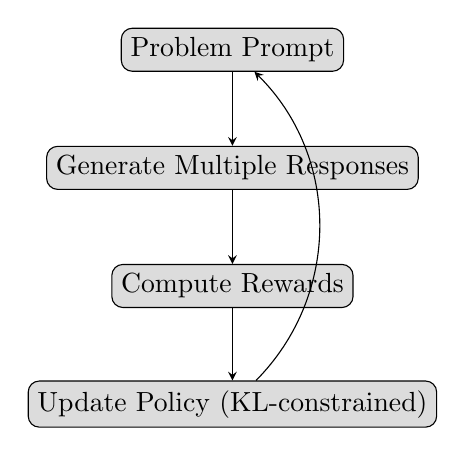
\begin{tikzpicture}[node distance=1.5cm]
      \node (prompt) [draw, rounded corners, fill=gemmagray!20] {Problem Prompt};
      \node (generate) [draw, rounded corners, fill=gemmagray!20, below of=prompt] {Generate Multiple Responses};
      \node (reward) [draw, rounded corners, fill=gemmagray!20, below of=generate] {Compute Rewards};
      \node (optimize) [draw, rounded corners, fill=gemmagray!20, below of=reward] {Update Policy (KL-constrained)};
      
      \draw[-stealth] (prompt) -- (generate);
      \draw[-stealth] (generate) -- (reward);
      \draw[-stealth] (reward) -- (optimize);
      \draw[-stealth] (optimize) to [bend right=45] (prompt);
    \end{tikzpicture}
  \end{center}
\end{frame}

\section{Reward Functions for Mathematical Reasoning}

\begin{frame}{Structuring Mathematical Answers}
  \begin{itemize}
    \item Special tokens for structured reasoning:
    \begin{itemize}
      \item \specialtoken{start\_reasoning} and \specialtoken{end\_reasoning}
      \item \specialtoken{answer} and \specialtoken{/answer}
    \end{itemize}
    \item Enables systematic evaluation of:
    \begin{itemize}
      \item Step-by-step reasoning process
      \item Final numerical answer
    \end{itemize}
    \item Example format:
    \begin{align*}
    &\specialtoken{start\_reasoning}\\
    &\text{To solve this problem, I'll first...}\\
    &\text{Step 1: Calculate...}\\
    &\text{Step 2: Apply the formula...}\\
    &\specialtoken{end\_reasoning}\\
    &\specialtoken{answer}42\specialtoken{/answer}
    \end{align*}
  \end{itemize}
\end{frame}

\begin{frame}{Multi-component Reward Function}
  \begin{itemize}
    \item Combined reward with weighted components:
    \begin{align*}
    R_{\text{total}} = w_f \cdot R_{\text{format}} + w_a \cdot R_{\text{answer}} + w_r \cdot R_{\text{reasoning}}
    \end{align*}
    \item Where:
    \begin{itemize}
      \item $R_{\text{format}}$: Rewards proper use of special tokens
      \item $R_{\text{answer}}$: Rewards numerical accuracy of final answer
      \item $R_{\text{reasoning}}$: Rewards quality of step-by-step explanation
      \item $w_f, w_a, w_r$: Adjustable weights for each component
    \end{itemize}
  \end{itemize}
\end{frame}

\begin{frame}{Format Reward}
  \begin{itemize}
    \item Two approaches for format evaluation:
    \begin{itemize}
      \item \textbf{Exact format matching}: Higher reward when all special tokens are present in correct order
      \item \textbf{Approximate format matching}: Partial reward based on token presence
    \end{itemize}
    \item Encourages model to adopt consistent response structure
    \item Aids in automated evaluation and parsing
    \item Score range: -2.0 to +3.0
  \end{itemize}
\end{frame}

\begin{frame}{Answer Reward}
  \begin{itemize}
    \item Evaluates correctness of the final answer
    \item Tiered scoring system:
    \begin{itemize}
      \item Perfect match: Highest reward (+3.0)
      \item Match after normalization: Medium reward (+1.5)
      \item Numerically close: Low reward (+0.5 to +0.25)
      \item Incorrect: Negative reward (-1.0)
    \end{itemize}
    \item Handles various answer formats:
    \begin{itemize}
      \item Exact string matching
      \item Numerical comparison with tolerance
      \item Digit-only comparison for special cases
    \end{itemize}
  \end{itemize}
\end{frame}

\begin{frame}{Reasoning Quality Reward}
  \begin{itemize}
    \item Evaluates the quality of step-by-step reasoning
    \item Features analyzed:
    \begin{itemize}
      \item \textbf{Length}: Longer reasoning tends to be more complete
      \item \textbf{Structured steps}: Presence of numbered steps or bullet points
      \item \textbf{Mathematical notation}: Use of symbols and equations
      \item \textbf{Multi-line work}: Evidence of thorough calculation
    \end{itemize}
    \item Encourages thorough, clear explanations
    \item Additive scoring system: 0.0 to +2.0
  \end{itemize}
\end{frame}

\section{Implementation Details}

\begin{frame}{Model Architecture}
  \begin{itemize}
    \item Gemma 3-4B core architecture:
    \begin{itemize}
      \item Transformer-based language model
      \item 4 billion parameters
      \item BFloat16 precision for TPU optimization
      \item Integration with JAX for efficient training
    \end{itemize}
    \item Special considerations for GRPO:
    \begin{itemize}
      \item Reference model (frozen) for KL divergence calculation
      \item Policy model (optimized) for response generation
      \item Chat sampling with temperature and top-k/top-p
    \end{itemize}
  \end{itemize}
\end{frame}

\begin{frame}{Checkpoint Structure}
  \begin{itemize}
    \item Orbax checkpoint management:
    \begin{itemize}
      \item Efficient storage of model parameters
      \item Metadata for tracking training state
      \item Compatibility with JAX ecosystem
    \end{itemize}
    \item Directory structure reflects JAX's parameter organization
    \item Manifests track parameter locations and versions
    \item Enables efficient parameter loading and saving
  \end{itemize}
\end{frame}

\begin{frame}{Training Hyperparameters}
  \begin{center}
    \begin{tabular}{lr}
      \toprule
      \textbf{Parameter} & \textbf{Value} \\
      \midrule
      Learning rate & 5e-6 \\
      KL coefficient & 0.1 \\
      Max gradient norm & 0.1 \\
      Generations per prompt & 4 \\
      Max sequence length & 1024 \\
      Format reward weight & 1.0 \\
      Answer reward weight & 2.0 \\
      Reasoning reward weight & 1.0 \\
      Adam $\beta_1$ & 0.9 \\
      Adam $\beta_2$ & 0.99 \\
      Weight decay & 0.1 \\
      \bottomrule
    \end{tabular}
  \end{center}
\end{frame}

\begin{frame}{Optimization Process}
  \begin{itemize}
    \item Process for each batch:
    \begin{enumerate}
      \item Generate multiple responses for each prompt
      \item Compute rewards for all responses
      \item Calculate policy gradient loss (maximize reward)
      \item Calculate KL divergence from reference model
      \item Combine losses with KL penalty
      \item Apply gradient updates with AdamW optimizer
      \item Clip gradients to prevent instability
    \end{enumerate}
    \item Cosine learning rate schedule with warmup
  \end{itemize}
\end{frame}

\section{Evaluation and Results}

\begin{frame}{Evaluation Metrics}
  \begin{itemize}
    \item Training metrics:
    \begin{itemize}
      \item Policy gradient loss
      \item KL divergence from reference model
      \item Mean reward across batches
      \item Response length distribution
    \end{itemize}
    \item Reward component analysis:
    \begin{itemize}
      \item Format score distribution
      \item Answer accuracy rate
      \item Reasoning quality metrics
    \end{itemize}
    \item Best and worst examples tracked for qualitative analysis
  \end{itemize}
\end{frame}

\begin{frame}{Sample Mathematical Reasoning}
  \textbf{Problem:} A train travels at 60 km/h for the first 150 km, then at 90 km/h for the next 180 km. What is the average speed for the entire journey?
  
  \vspace{0.3cm}
  \footnotesize
  \texttt{<start\_reasoning>}
  
  To solve this problem, I need to find the total distance and total time.
  
  Total distance = 150 km + 180 km = 330 km
  
  Time for first segment = Distance ÷ Speed = 150 km ÷ 60 km/h = 2.5 h
  
  Time for second segment = 180 km ÷ 90 km/h = 2 h
  
  Total time = 2.5 h + 2 h = 4.5 h
  
  Average speed = Total distance ÷ Total time = 330 km ÷ 4.5 h = 73.33 km/h
  
  \texttt{<end\_reasoning>}
  
  \texttt{<answer>}73.33 km/h\texttt{</answer>}
\end{frame}

\begin{frame}{Summary and Future Work}
  \begin{itemize}
    \item GRPO successfully improves Gemma 3-4B's mathematical reasoning
    \item Multi-component reward functions provide targeted guidance
    \item Efficient implementation with JAX enables training on TPUs
    \item Future directions:
    \begin{itemize}
      \item Expanding to more complex mathematical domains
      \item Incorporating multimodal inputs for visual math problems
      \item Adaptive reward weighting based on problem difficulty
      \item Exploring alternative policy optimization techniques
      \item Scaling to larger model variants
    \end{itemize}
  \end{itemize}
\end{frame}

\begin{frame}{Conclusion}
  \begin{center}
    \Large Thank you!
    
    \vspace{0.5cm}
    \normalsize Questions?
  \end{center}
\end{frame}

\end{document}